
\section{Estimating the Spatial Closure from the HO Solution}
\label{sec:spat_clos}

REWRITE: Some of this could maybe be moved to the introduction
This sections describes an alternative spatial closure to the LO equations based on 
a parametric relation from the HO solution. In addition to estimating the angular
consistency terms, the HO intensity estimates a relation between volume and face-averaged
intensities to eliminate the remaining unknowns from the equations.  The goal is for the 
LO moments to reproduce the HO moments more accurately than the LDFE discretization, although
additional statistical noise is introduced through face-based tallies.  In the remainder of this section, we will motivate the HO spatial closure by forming half
range balance equations to form a single unknown for each cell.  We will then discuss
possible closure relations, based on modifications to standard spatial closures.

\subsection{Motivation}

A half-range balance equation for $\mu>0$ is formed by adding the
exact $L$ and
$R$ radation moment equations given by
Eq.~\eqref{eq:exact_lmomp}~and~\eqref{eq:exact_rmomp}, i.e.,
\begin{equation}\label{eq:hr_bal}
    \overline\mu^+_{i+1/2}\phi_{i+1/2}^+ - \overline\mu^+_{i-1/2}\phi_{i-1/2}^+ +
    {\sigma_{a,i}h_i} \phi_i^+ = \frac{h_i}{2} q_i,
\end{equation}
where $q_i$ represents the cell-average of all isotropic source terms.  In the HOLO
method, to reduce the number of unknowns, the
angular consistency terms are estimated
with the previous HO solution.  Additionally, the inflow term $\phi_{i-1/2}^+$ is eliminated via upwinding from the previous
cell or a boundary condition.  An additional equation is needed to eliminate the outflow $\phi_{i+1/2}^+$ to produce an
equation for a single unknown $\phi_{i}^+$.  Standard spatial discretizations techniques
use a fixed approximation for all cells to eliminate the outflow in terms of other
unknowns.  Alternatively, the HO solution can be used to estimate a parametric relation
between the other uknowns and the outflow, i.e.,
\begin{equation}
    \phi_{i+1/2}^+ = f(\gamma^{HO}_i, \phi_i^+, \phi_{x,i}^+, \phi_{i-1/2}^+).
\end{equation}
Here, $\gamma^{HO}_i$ is a constant estimated with the HO solution and $f$ is some
function of some number of the input
variables.  The ECMC solution can provide all of the unknowns in the above equation, so
the value of $\gamma^{HO}_i$ can be determined.

If the problem were linear, or the nonlinear problem was fully converged,
then application of this closure can ensure that the HO and LO equations produce the same moments.  To produce the
same moments, the HO solution must also satisfy the local balance equation, e.g.,
Eq.~\eqref{eq:hr_bal}.  If any higher moments are introduced through the spatial closure,
then the HO solution must also satisfy the same relations as the LO equations.  For example, both the LO and HO equation must satisfy the
first moment equation in space if the closure is a function of the first moment.  
then the HO and LO solutions would produce exactly the same moments.  There are
several issues with ECMC that cause this to not be true, even for a linear problem.
With ECMC, global and, particularly, local energy balance are not preserved.  There
are source biasing techniques for standard MC (e.g., systematic
sampling) that exactly preserve the zeroth moment of the
source~\cite{shultis_mc,wollaber_review}). 
However, because we have to reconstruct the bilnear moment
of $x$ and $\mu$, the consistency terms do not exactly preserve the first moment
equation.  One final reason is that the analog treatment of absorption (below the weight
cutoff, as discussed in Sec.~\ref{???}) results in $\sigma_a \phi^{HO}_i$ and the amount
of energy removed from a cell during MC transport to not be equal, due to statistical noise in the
path-length estimators for $\phi^{HO}_i$.  However, ECMC will preserve
balance to the order of the error, so the closure parameters will
reproduce the HO moments to the accuracy of the LO solution.

REWRITE:  THIS IS SAYING WHY LDFE PROJECTION AND LDFE-DISCRETI ZATION ARE NOT EQUAL,
PROBALBY JUST DELETE
It is noted that the LD projection of the HO solution does not produce the same moments, because
MC was used to obtain this projection, the outflow will not agree with the LO equations.
For example, the upwinding inflow from a previous cell does not match the actual energy
that flowed through that surface due to MC noise.



As TRT problems are non-linear (i.e., scattering or thermal emission are included in
$q$), the moments will only be preserved upon non-linear convergence of the source.  The
nonlinearity introduces the possibility for stability
issues, particularly with MC noise.  However, we have already consistently formed angular consistency terms, so the
the spatial closure should be more stable than introducing other terms, such as
in NDA methods. 


%THIS SENTENCE WAS REDUNDANT I THINK, BUT GOOD
REWRITE: MAYBE IT SHOULD GO IN THE INTRO
After approximating the angular consistency terms in the time-discretized LO moment equations, 
there is still more unknowns than equations, for each spatial
cell and half range; an extra equation relating the spatial moments and outflow face values is
needed, i.e., a spatial closure.

\subsection{Choice of Spatial Closure}
\label{sec:spat_clos_options}

We will
explore two different closure relations: a scaled slope, i.e.,
\begin{equation}
    \phi_{i\pm1/2}^\pm = \phi_i^+ \pm \gamma_i \phi_{x,i}^+
\end{equation}
and a scaled average
\begin{equation}
    \phi_{i\pm1/2}^\pm = \gamma_i \phi_i^+ \pm \phi_{x,i}^+,
\end{equation}
where a value of $\gamma_i = 1$ produces the standard linear discontinuous expressions for
the extrapolated outflows.  

We now use the HO solution to estimate $\gamma_i$.  For example, 
\begin{equation}
    \gamma_i^{+,HO} = \frac{\phi_{i+1/2}^+ - \phi_{x,i}^+}{\phi_i^+}
\end{equation}
in the scaled slope case.  For this closure, as the slope goes to zero this expression
becomes undefined.  In cells where the slope is $O(10^{-13} \psi_i)$, we use $\gamma_i=1$.
For the problems tested, no issues have occurred with this closure, even $\gamma$
can become very large for common, small values of $|\psi^x/\psi_i|$.  This is because in
such regions the solution is changing minimally anyways. 
The main benefit of this closure is it allows for values of $\gamma$ that are
equivalent to step ($\gamma_i=0$) and lumped ($\gamma_i=1/3$) expressions.

To solve the LO equations, the expression for the outflow face term is substituted in each equation, using the
$\gamma_i$ estimated from the HO solution. There is a spatial closure parameter for each
half-range, for each cell.
For instance, the positive balance equation becomes
\begin{equation}
    \overline\mu^+_{i+1/2}\left( \gamma_i^{+,HO} \phi_i^+ + \phi_{x,i}^+ \right) - \overline\mu^+_{i-1/2}\phi_{i+1/2}^+ +
    \frac{\sigma_{a,i}h_i}{2} \phi_i^+ = \frac{h_i}{2} q_i,
    \label{eqn:clsd_posbal}
\end{equation}
noting that $\phi_i^+$ and $\phi_{x,i}^+$ remain as unknowns. The MC solution must be modified
to tally the solution on faces. Our LO system is formulated in terms of $L$ and $R$ moments, rather than the average and
slope.  Thus, the parameteric functions are expressed in terms of the $L$ and $R$
unknowns, using the relations given in App.~\ref{app:lo_mom_relations}.  


\subsection{The Doubly-Discontinuous Trial Space}

Because of the temperature unknowns and the HO scattering source representation, a
representation on the interior of the cell for the temperature and intensity is needed.
However, the outflow from the cell is now a parametric (i.e., non linear)
extrapolation of the interior moments. Thus, we introduce a linear doubly
discontinuous (LDD) trial space for the half-range intensities, which is depicted in Fig.~\ref{fig:ldd_space}.
The linear relation on the interior of the cell preserves the $L$ and $R$ moments of the
solution.  The temperature is still represented with a linear interpolant of $T^4$ and
$T$.  
This trial space has an extra unknown outflow, which is eliminated using the HO spatial
closure.  For the initial LO solve, the outflow is assumed continuous, using the standard
upwinding and LD representation.  With the outflow term eliminated, the equations
have the same numerical complexity as the LD equations.   

In the case of strong gradients, the interior representation could be driven
negative.  Thus, we use the lumped expression to to define the linear representation.  For
example, the lumped emission source is
\begin{equation}
    T = \mom{T}_{L,i}^4 b_{L,i}(x) + \mom{T}_{R,i}^4 b_{R,i}(x) , \quad x\in(\xl,\xr)
\end{equation}
This expression is positive as long as the moments are positive, which is true for
physical solutions.  If the lagged, MC spatial closure produces an outflow from a cell that is
negative, then these moments could become negative.  In such cases, we force that cell to
use a standard lumped relation for the moment equations, with no discontinuity at the
outflow.  As verified in Sec.~\ref{sec:sec_order}, the interior solution is still second
order accurate in space.

During the Newton solve, once new half-range
intensities are determined, the temperatures are updated using the moment same moment
equations given by Eq.~\eqref{}. This can be confusing because the slope moment,
e.g., $\psi_{x,i}^\pm$, does not stricly correspond to the slope in the typical since.
We have modified it.  This is the same as the lumped closure relation using
$\gamma_i=1/3$, where we are preserving the average moment exactly, but only second order
accurate in the slope.


\begin{figure}[H]
    \centering
    \begin{center}
        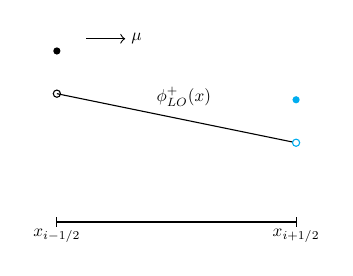
\begin{tikzpicture}[scale=0.62, every node/.style={transform shape}]
            \draw (1.0,4.0) node[fill,circle,inner sep=0pt,minimum
            size=4.2pt] {};
            \draw [->] (1.6,4.25) -- (2.4,4.25) node[anchor=west] {$\mu$};
            \draw (1.0,0.4) -- (1.0,0.6) node[below, pos=0.4] {$x_{i-1/2}$};
            \draw (5.90,0.4) -- (5.90,0.6) node[below, pos=0.4] {$x_{i+1/2}$};
            \node at (3.6,3.06) {$\phi_{LO}^+(x)$};
            \draw [thick] (1.0,0.5) -- (5.9,0.5) node[anchor=north west] {};
            \filldraw[color=black, fill=white] (1,3.1250) circle (2.1pt);
            \draw (1.0,3.125) -- (5.90,2.120);
            \filldraw[color=cyan, fill=white] (5.9,2.120) circle (2.1pt);
            \draw (5.9,3.0) node[cyan,fill,circle,inner sep=0pt,minimum size=4.2pt] {};
        \end{tikzpicture}
    \end{center}
    \caption{Linear doubly-discontinous representation for mean intensity in LO equations}
    \label{fig:ldd_space}
\end{figure}

Poor statistics for the face tallies may result in this trial space producing less
accurate results compared to the standard LDFE solution, at least for sufficiently fine meshes where LD
can accurately represent the solution.  Although the closure will be applied everywhere,
we expect the greatest improvement in accuracy for cells where the LDFE trial space
produces a negative solution.

\section{Test Problems}

REWRITE: I THINK MOVE THIS TO THE INTRO SOME HOW
To investigate the utility of the face closures we compare to the LD spatial
closure for two simple test problems.  We are interested in the accuracy of the solution. 
We also want to demonstrate a better consistency between the two solvers, particularly at
coarser mesh sizes.  We also want to compare to the efficiency of LD, noting that the
extra noise of the face tallies may make the solution approach not worth it over all.

\subsection{Smooth Marshak Wave}

The first problem is intended to have a relatively smooth solution, as well as cells that
are not too optically thick so that the face-based solutions can be efficiently estimated.
For this problem we use


